\documentclass{article}

\usepackage{graphicx}
\usepackage{tikz}
\usepackage{tikzsymbols}
\usetikzlibrary{calc,patterns,shapes.geometric}
\pagestyle{empty}
\usepackage[margin=0pt]{geometry}
\geometry{papersize={14in,12in}}

\def\centerarc[#1](#2)(#3:#4:#5){\draw[#1] ($(#2)+({#5*cos(#3)},{#5*sin(#3)})$) arc (#3:#4:#5);}

\begin{document}
	\begin{figure}
		\centering
		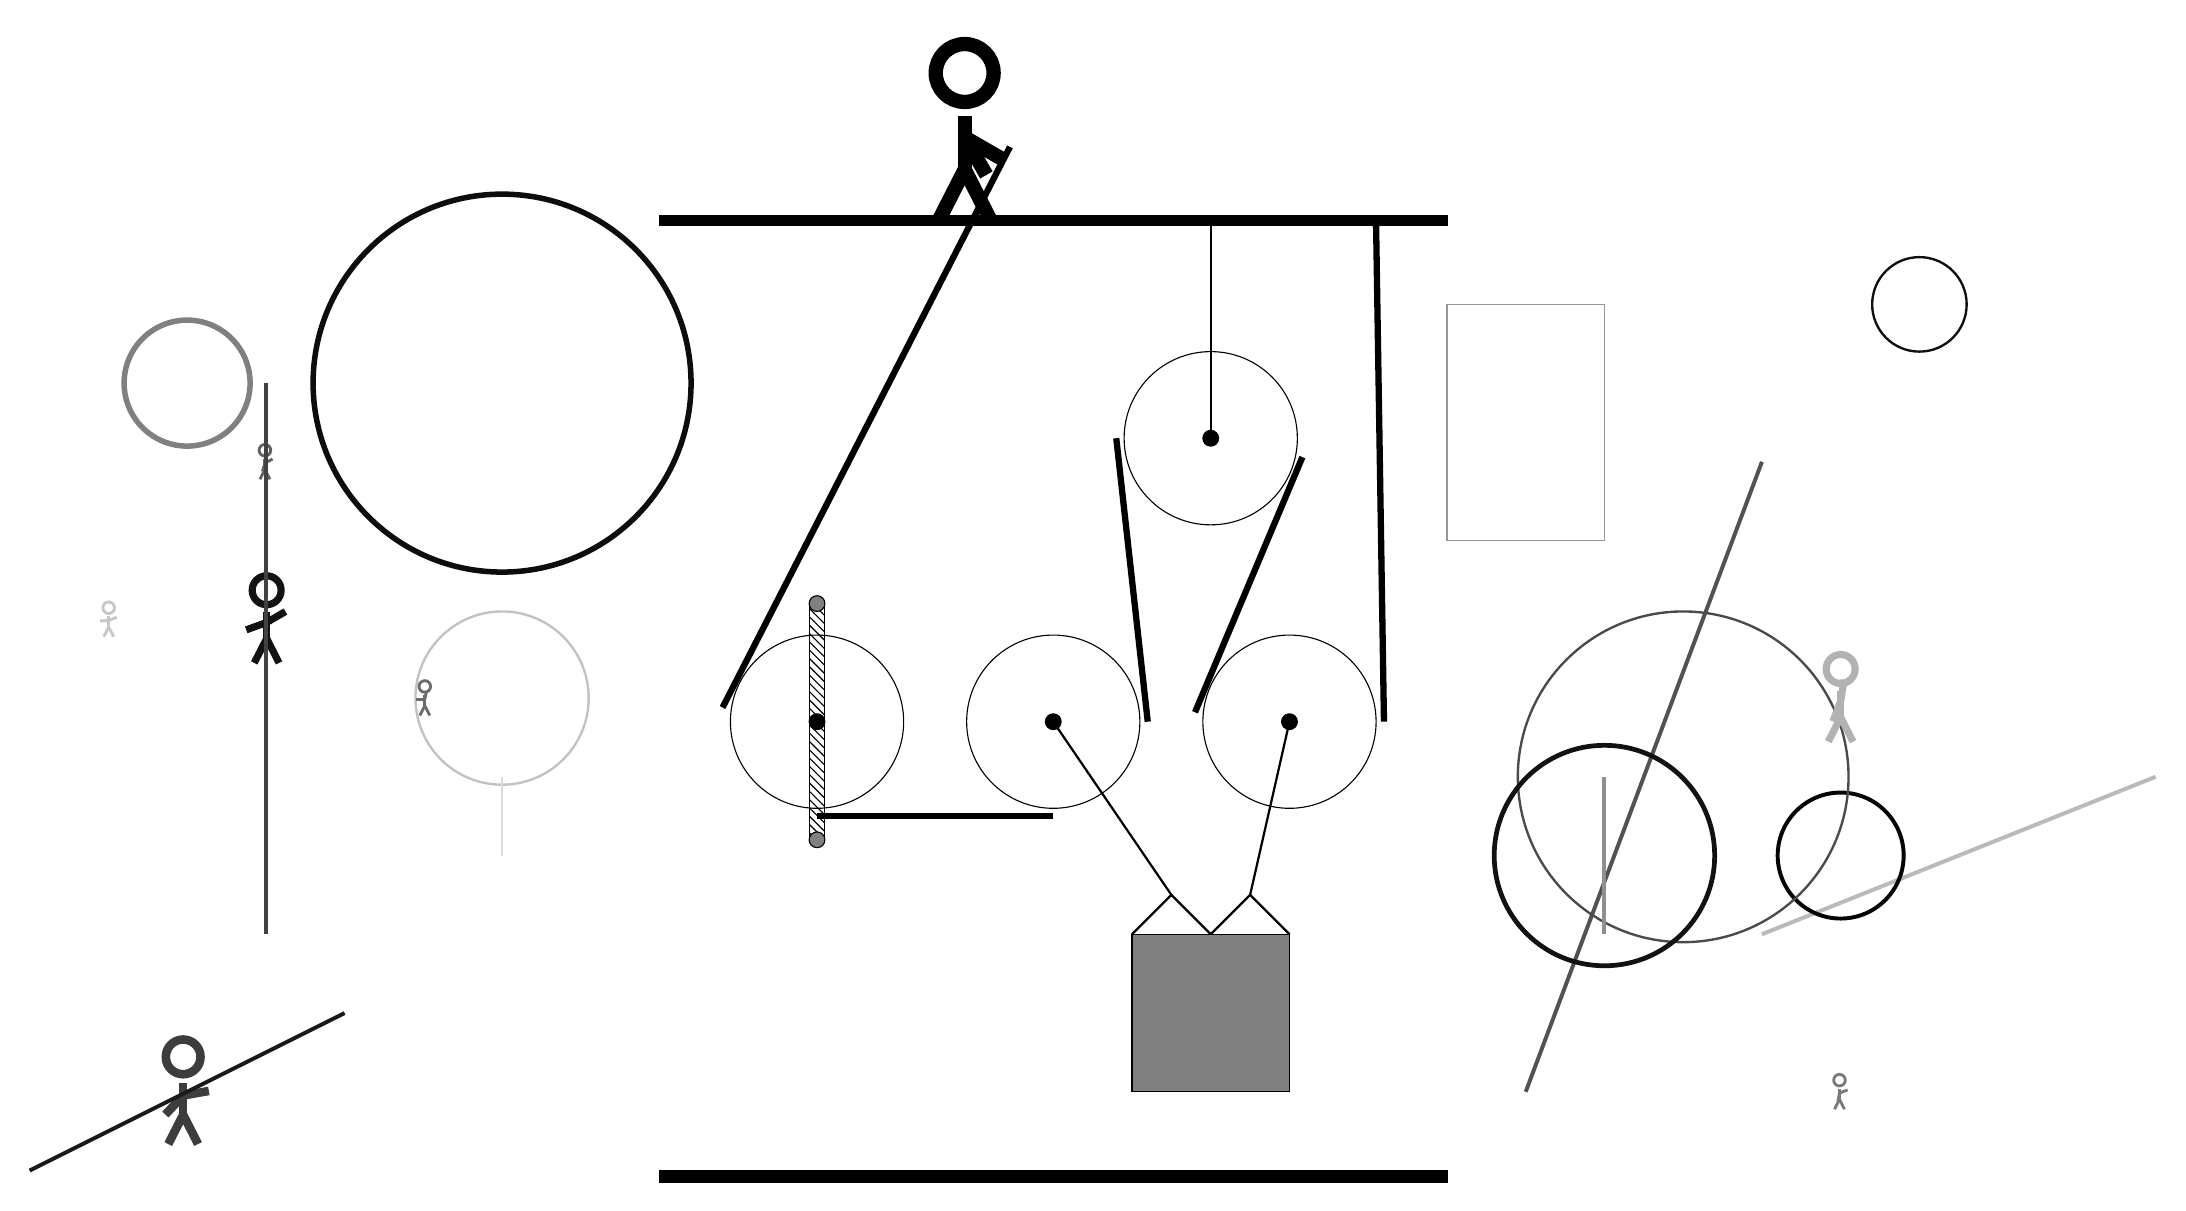
\begin{tikzpicture}
			%%%%% START %%%%%
			
			\draw[fill=black] (-4, 9) rectangle (6, 9.125);
			
			\draw (1, 2.7) circle (1.1);
			\draw[fill=black] (1, 2.7) circle (0.1);
			
			\draw (3, 6.3) circle (1.1);
			\draw[fill=black] (3, 6.3) circle (0.1);
			\draw[thick] (3, 6.3) -- (3, 9);
			
			\draw (4, 2.7) circle (1.1);
			\draw[fill=black] (4, 2.7) circle (0.1);
			
			\draw [line width=0.3mm, color=black!24](-6, 3) circle (1.1);
			
			\node[line width=0.5mm, color=black!93] at (-9, 4) {\Strichmaxerl[5][20][30]};
			\draw[line width=0.5mm, color=black!27](10, 0) -- (15, 2);
			\node[line width=0.3mm, color=black!76] at (-10, -2) {\Strichmaxerl[6][47][10]};
			\draw [line width=0.5mm, color=black!99](11, 1) circle (0.8);
			
			\node[line width=0.2mm, color=black!22] at (-11, 4) {\Strichmaxerl[2][2][23]};
			
			\node[line width=0.3mm, color=black!62] at (-9, 6) {\Strichmaxerl[2][73][28]};
			\draw[line width=0.5mm, color=black!68](10, 6) -- (7, -2);
			\draw[line width=0.2mm, color=black!41] (6, 5) rectangle (8, 8);
			\draw[line width=0.5mm, color=black!74](-9, 0) -- (-9, 7);
			
			\draw [line width=0.3mm, color=black!71](9, 2) circle (2.1);
			
			\node[line width=0.2mm, color=black!52] at (11, -2) {\Strichmaxerl[2][79][21]};
			\draw[line width=0.5mm, color=black!44](8, 2) -- (8, 0);
			
			\node[line width=0.7mm, color=black!30] at (11, 3) {\Strichmaxerl[5][69][81]};
			\draw [line width=0.7mm, color=black!50](-10, 7) circle (0.8);
			\draw [line width=0.7mm, color=black!95](-6, 7) circle (2.4);
			\draw[line width=0.5mm, color=black!90](-8, -1) -- (-12, -3);
			\draw [line width=0.6mm, color=black!93](8, 1) circle (1.4);
			\node[line width=0.2mm, color=black!58] at (-7, 3) {\Strichmaxerl[2][0][78]};
			\draw [line width=0.3mm, color=black!94](12, 8) circle (0.6);
			\draw[line width=0.3mm, color=black!14] (-6, 2) rectangle (-6, 1);
			
			
			\draw[thick] (4, 2.7) -- (3.5, 0.5);
			\draw[thick] (1, 2.7) -- (2.5, 0.5);
			\draw[thick]  (2, 0) -- (2.5, 0.5) -- (3, 0);
			\draw[thick]  (3, 0) -- (3.5, 0.5) -- (4, 0);
			\draw[fill=black!50] (2, 0) rectangle (4, -2);
			
			\draw (-2, 2.7) circle (1.1);
			\draw[fill=black] (-2, 2.7) circle (0.1);
			\draw[pattern=north west lines, pattern color=black] (-2.1, 4.2) rectangle (-1.9, 1.2);
			\draw[fill=black!50] (-2, 4.2) circle (0.1);
			\draw[fill=black!50] (-2, 1.2) circle (0.1);
			
			\draw[line width=0.8mm] (0.45, 10) -- (-3.2, 2.88);
			\centerarc[line width=0.8mm](-2, 2.7)(160:270:1.2000000000000002);
			\draw[line width=0.8mm](-2, 1.5) -- (1, 1.5);
			\centerarc[line width=0.8mm](1, 2.7)(270:360:1.2000000000000002);
			\draw[line width=0.8mm] (2.2, 2.7) -- (1.8, 6.3);
			\centerarc[line width=0.8mm](3, 6.3)(-20:180:1.2000000000000002);
			\draw[line width=0.8mm](4.164, 6.06) -- (2.8, 2.82);
			\centerarc[line width=0.8mm](4, 2.7)(160:360:1.2000000000000002);
			\draw[line width=0.8mm](5.2, 2.7) -- (5.1, 9);
			
			\node at (-0.07, 10.2) {\Strichmaxerl[10][120][-30]};
			
			\draw[fill=black] (-4, -3) rectangle (6, -3.15);
			
			%%%%% END %%%%%
		\end{tikzpicture}
	\end{figure}	
\end{document}